% Created 2024-07-07 Sun 22:55
% Intended LaTeX compiler: xelatex
\documentclass[a4paper,11pt,twoside]{article}
\usepackage{graphicx}
\usepackage{longtable}
\usepackage{wrapfig}
\usepackage{rotating}
\usepackage[normalem]{ulem}
\usepackage{amsmath}
\usepackage{amssymb}
\usepackage{capt-of}
\usepackage{hyperref}
\usepackage{libertine} \usepackage{amsmath}
\usepackage[width=200.00mm, height=240.00mm, left=3cm, right=3cm, top=3 cm, bottom=3cm]{geometry}
\usepackage{graphicx}
\graphicspath{ {./images/} }
\usepackage{multicol}
\author{Ryan P. Lynch}
\date{\today}
\title{Program 1B}
\hypersetup{
 pdfauthor={Ryan P. Lynch},
 pdftitle={Program 1B},
 pdfkeywords={},
 pdfsubject={},
 pdfcreator={Emacs 29.3 (Org mode 9.6.24)}, 
 pdflang={English}}
\usepackage{biblatex}

\begin{document}

\maketitle
\section*{Compile and Executing}
\label{sec:orgcbb6596}
\begin{document}
The screenshot below shows the compiling of Shell.java\\
It also shows the testing of concurrent commands. All three PingPong commands are ran at the same time, having their outputs mixed in with each others.\\
\centerline{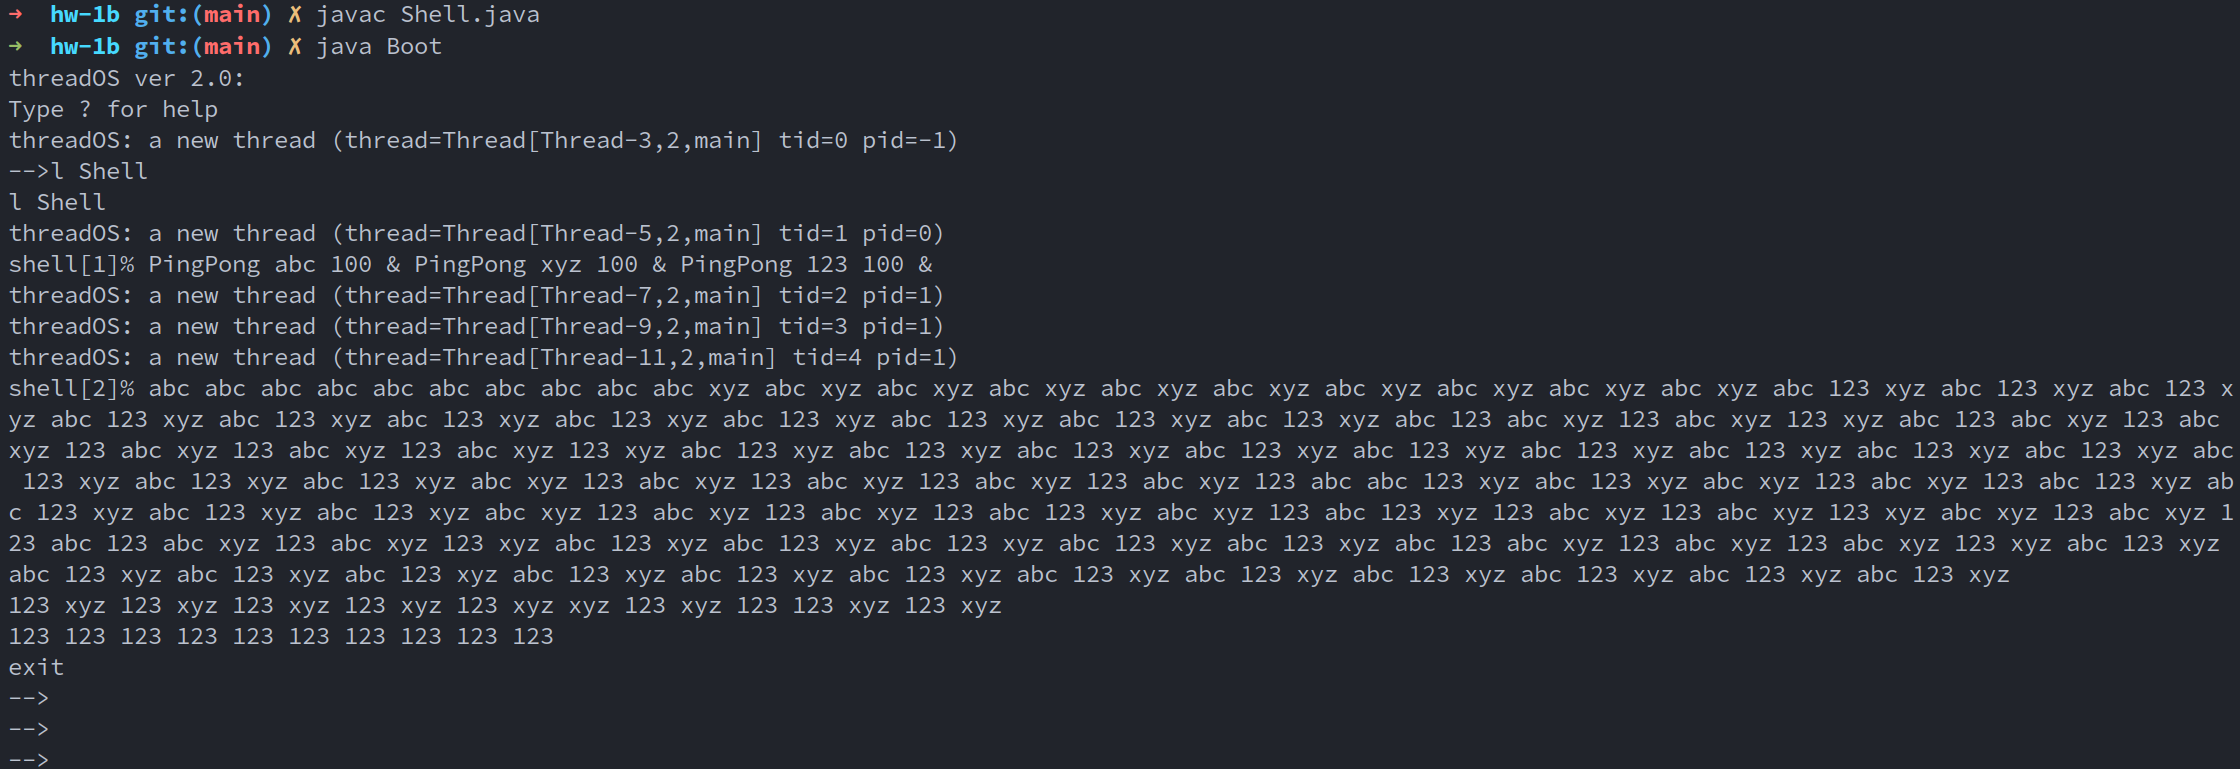
\includegraphics[scale=.35]{conurrent-test}}
\\
\\
The screenshot below shows the compiling of Shell.java\\
It also shows the testing of sequential commands. Each PingPong command must wait for the previous one to finish before it is allowed to create a thread start running.\\
\centerline{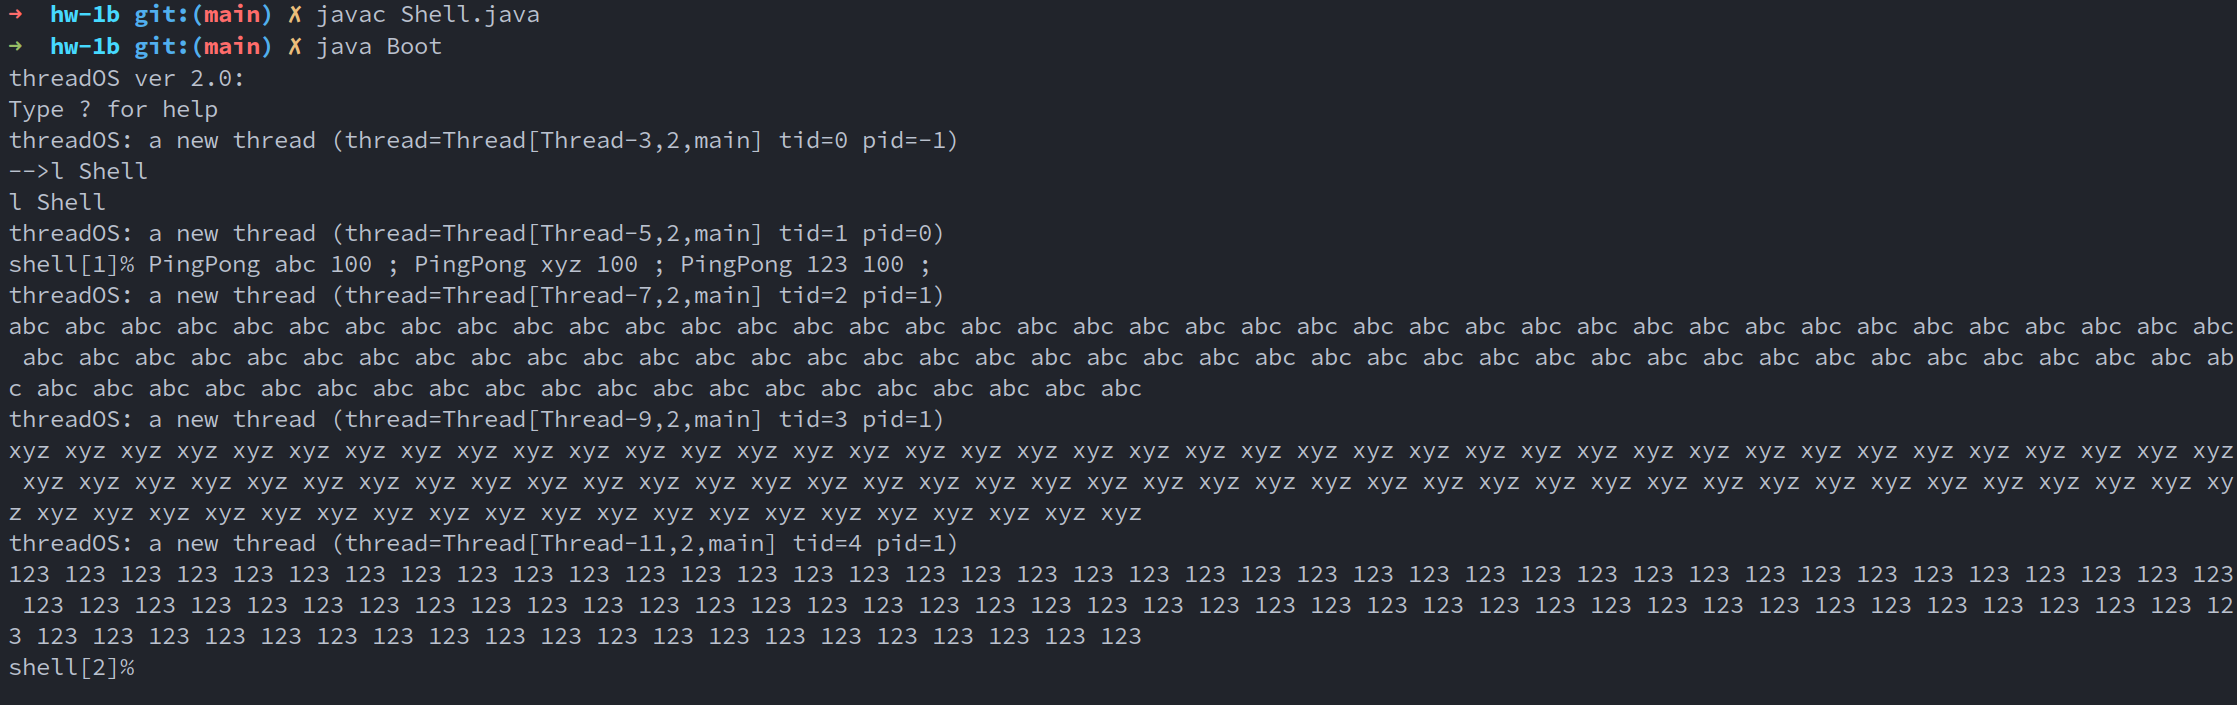
\includegraphics[scale=.35]{sequential-test}}
\end{document}
\end{document}
